\documentclass{standalone}
\usepackage{pgf-umlcd}
\begin{document}
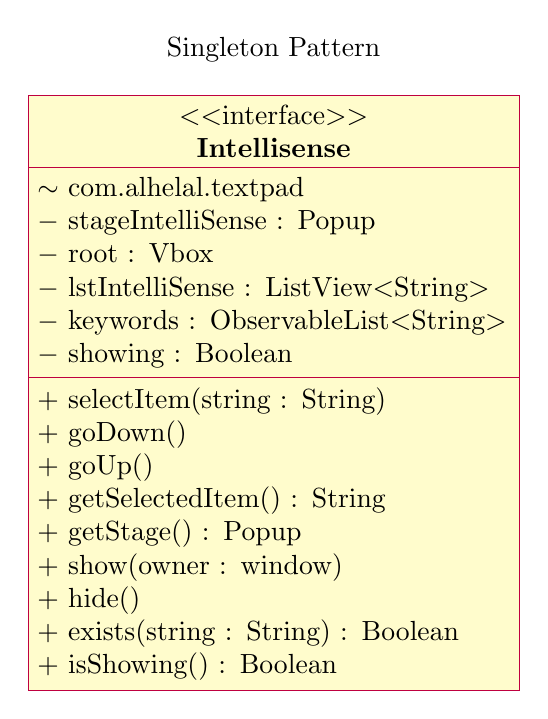
\begin{tikzpicture}

  \begin{interface}[text width = 6cm]{Intellisense}{0,0}
    \attribute{$\sim$ com.alhelal.textpad}
    \attribute{$-$ stageIntelliSense : Popup}
    \attribute{$-$ root : Vbox}
    \attribute{$-$ lstIntelliSense : ListView$<$String$>$}
    \attribute{$-$ keywords : ObservableList$<$String$>$}
    \attribute{$-$ showing : Boolean}
    \operation{+ selectItem(string : String)}
    \operation{+ goDown()}
    \operation{+ goUp()}
    \operation{+ getSelectedItem() : String}
    \operation{+ getStage() : Popup}
    \operation{+ show(owner : window)}
    \operation{+ hide()}
    \operation{+ exists(string : String) : Boolean}
    \operation{+ isShowing() : Boolean}
\end{interface}
  \node [above=3mm] at (current bounding box.north) {Singleton Pattern};
\end{tikzpicture}
\end{document}
